\documentclass[12pt,a4paper]{article}
\usepackage{amsmath, amssymb, bm, empheq, geometry, graphicx, hyperref, mhchem, multirow, siunitx, subcaption, upgreek}
\usepackage[italicdiff]{physics}
\usepackage[section]{placeins}
\usepackage[justification=centering]{caption}
\usepackage[extrafootnotefeatures]{xepersian}

\hypersetup{colorlinks=true, urlcolor=cyan}
\settextfont{Yas}
\ExplSyntaxOn
\cs_set_eq:NN
\etex_iffontchar:D
\tex_iffontchar:D
\cs_undefine:N \c_one
\int_const:Nn \c_one { 1 } 
\ExplSyntaxOff
\setdigitfont{Yas}

\title{محاسبه غیر مستقیم زمان واپاشی ذرات}
\author{حسین حاتم‌نیا، صالح شاملو احمدی\\دانشگاه صنعتی شریف، دانشکده فیزیک}

\begin{document}
	\maketitle
	\begin{abstract}
		زمان رخداد بسیاری پیدیده‌های فیزیکی به صورت مستقیم قابل اندازه‌گیری نیست. به عنوان مثال نیمه‌عمر کربن-۱۴ حدود $5700$ سال و زمان واپاشی ذرات
		از کانال برهم‌کنش قوی از مرتبه $10^{-23}$ ثانیه است. در ادامه بررسی می‌کنیم که چطور می‌توانیم به صورت غیر مستقیم این مقادیر را محاسبه کنیم.
		پاسخ کوتاه این است که با تعمیم دانشی که از بازه‌های زمانی قابل اندازه‌گیری داریم، الگویی پیدا کنیم که بتوانیم با استفاده از آن مقادیر مربوط
		به بازه‌های زمانی بلندتر و کوتاه‌تر را پیشبینی کنیم. محوریت اصلی مقاله زمان‌های واپاشی کوتاه است، اما به زمان‌های بلندتر هم اشاره می‌کنیم.
	\end{abstract}
	\section{مقدمه}
	به طور معمول، اندازه‌گیری‌ها با مقایسه دو مقدار مختلف با هم انجام می‌گیرند؛ به عنوان مثال، برای اندازه‌گیری طول، فاصله خاصی را به عنوان «واحد» خود در نظر
	می‌گیریم و سپس برای اندازه‌گیری طول دلخواه‌مان، آن را در کنار واحد خود قرار می‌دهیم و بررسی می‌کنیم نسبت آن طول به واحدمان چقدر است. به طور خاص، چند
	«سانتی‌متر» روی یک خط‌کش را در کنار یک جسم قرار می‌دهیم و مقایسه می‌کنیم که ببینیم چندتا از این فاصله برابر طول یک جسم است.
	
	مسئله این است که برای اندازه‌گیری هر مقداری نمی‌توانیم آن را به طور مستقیم با مقداری در دسترس مقایسه کنیم. مثلاً خط‌کشی نداریم که در کنار فاصله زمین تا
	خورشید قرار دهیم تا ببینیم چند «متر» در آن جا می‌گیرد. مجبوریم از روشی غیر مستقیم، با استفاده از تعمیم الگویی خاص آن را پیدا کنیم. در این مورد، مشاهده
	می‌کنیم در بازه‌های کوتاه‌تر موج رادیویی سرعت ثابتی دارد. با اندازه‌گیری آن و فرض اینکه در فاصله زمین و خورشید هم موج رادیویی همین سرعت را حفظ می‌کند، و
	اندازه‌گیری زمانی که طول می‌کشد موج از خورشید بازتاب کند و به زمین برگردد، می‌توانیم فاصله را محاسبه کنیم. مثالی دیگر نیمه‌عمر مواد رادیواکتیو است که
	در برخی موارد به چند هزار سال می‌رسد. در این حالت با اندازه‌گیری جرم در بازه‌زمانی کوتاه‌تر، جرم بازه‌های زمانی بزرگ‌تر را برون‌یابی\footnote{extrapolate}
	می‌کنیم. یعنی با فرض اینکه فرایند واپاشی در بازه‌های زمانی طولانی‌تر، الگوی مشابهی را دنبال می‌کند، اندازه جرم در زمان‌های طولانی‌تر و در نتیجه نیمه‌عمر را
	پیش‌بینی می‌کنیم. در بازه‌های زمانی کوتاه‌تر می‌بینیم که به‌طور نمایی جرم کاهش پیدا می‌کند، و با پیدا کردن ضریب این افت نمایی جرم، نیمه‌عمر بدست می‌آید.
	سازگاری این روش‌ها با روش‌های دیگر در حالاتی که استفاده از روش‌های دیگر ممکن باشد و همچنین به مشکل نخوردن در توصیف فیزیکی، به ما این اطمینان را می‌دهند
	که این روش‌ها مشکلی ندارند. 
	
	برای ذرات با انرژی بالا، زمان برخی واپاشی‌ها با استفاده از دقیق‌ترین زمان‌سنج‌ها هم امکان‌پذیر نیست. برای بعضی ذرات می‌توانیم با توجه به انرژی، سرعت‌شان را
	اندازه‌گیری کنیم و با تقسیم طول ردّی که به جا می‌گذارند به مقدار بدست آمده برای سرعت، و البته اعمال اصلاحات نسبیتی، طول عمر را محاسبه کنیم. اما برای
	بعضی ذرات حتی این روش هم ممکن نیست؛ زمان واپاشی از کانال قوی از مرتبه $10^{-23}$ ثانیه است، و حتی اگر ذره با سرعت نور حرکت کند، از مرتبه بزرگی قطر یک
	پروتون (فمتومتر یا $10^{-15}$ متر) قبل واپاشی حرکت می‌کند. برای این ذرات، می‌توانیم از اصل عدم قطعیت استفاده کنیم.
	\section{اصل عدم قطعیت}
	طبق اصل عدم قطعیت انرژی-زمان (\cite{griffiths_schroeter_2018}، بخش ۳.۵.۳)
	\begin{equation}
	\Delta{E}\Delta{t} \ge \frac{\hbar}{2};
	\end{equation}
	در این رابطه $\Delta{E}$ انحراف معیار انرژی اندازه‌گیری شده ذرات و $\Delta{t}$ زمان مورد نیاز برای تغییر مقدار چشم‌داشتی یک مشاهده‌پذیر به اندازه انحراف
	معیار خود است. این به تعبیری طول‌عمر یک حالت کوانتومی است، که در اینجا همان طول‌عمر ذره یا زمان واپاشی است (حالت کوانتومی مربوط به یک ذره با واپاشی آن
	تغییر می‌کند). پس اگر انحراف معیار جرم‌های اندازه‌گیری شده برای ذره $\Delta{m}$ و زمان واپاشی $\tau$ باشد،
	\begin{equation}
		\tau \ge \frac{\hbar}{2\Delta{m}c^2}.
	\end{equation}
	البته این فقط یک حد پایین برای طول‌عمر است، اما چون نزدیک به حد کوانتومی شده‌ایم، طول‌عمر در همین مرتبه بزرگی است (به هر حال این تعریف از طول‌عمر هم
	مقدار دقیقی را نشان نمی‌دهد، بلکه وصفی تقریبی از پایداری این ذرات است).
	 
	حتی با این تعریف هم مشکل کامل حل نمی‌شود، فقط به اندازه‌گیری جرم‌ها منتقل می‌شود: چطور می‌توانیم جرم این ذرات را اندازه‌گیری کنیم؟ برای ذراتی که از خود
	رد به جا می‌گذارند، می‌توانیم از شعاع حرکت سیکلوترونی جرم را بدست بیاوریم، اما در اینجا ردی نداریم. پاسخ این است که باید از طریق آزمایش‌های رزونانس و
	سطح مقطع پراکندگی، یا با توجه به انرژی و تکانه ذرات تولید شده در واپاشی (که قابل اندازه‌گیری است)، آن را غیرمستقیم محاسبه کنیم.
	\section{از پراکندگی رادرفورد تا طول عمر ذرات بنیادی }
	مرجع: \cite{deoliveirasantos2018}
	
	رادرفورد در سال 1909 با مطالعه ی پراکندگی الاستیک ذرات باردار توسط نیروی دافعه ی کلمبی، نشان داد سطح مقطع دیفرانسیلی با عکس مجذور انرژی رابطه دارد.
	\begin{equation}\label{defcros}
		\frac{d\sigma}{d\Omega}=(\frac{Z_1Z_2e^2}{E \sin(\frac{\theta}{2})})^2
	\end{equation}
	
	که در آن $Z_2$ بار هدف، $E$ و $Z_1$ انرژی و بار ذره هستند. این مطالعه‌ها روی اتم‌های سنگین انجام شد و هنوز تب ذرات بنیادی شروع نشده بود.\\
	در آزمایش رادرفورد از ذرات آلفا استفاده شد و با ثابت نگه‌داشتن $\theta$ و رسم سطح مقطع دیفرانسیلی بر حسب انرژی، انتظار داریم نمودار مانند شکل
	\ref{fig:diffcross} شود.
	
	\begin{figure}[h]
		\centering
		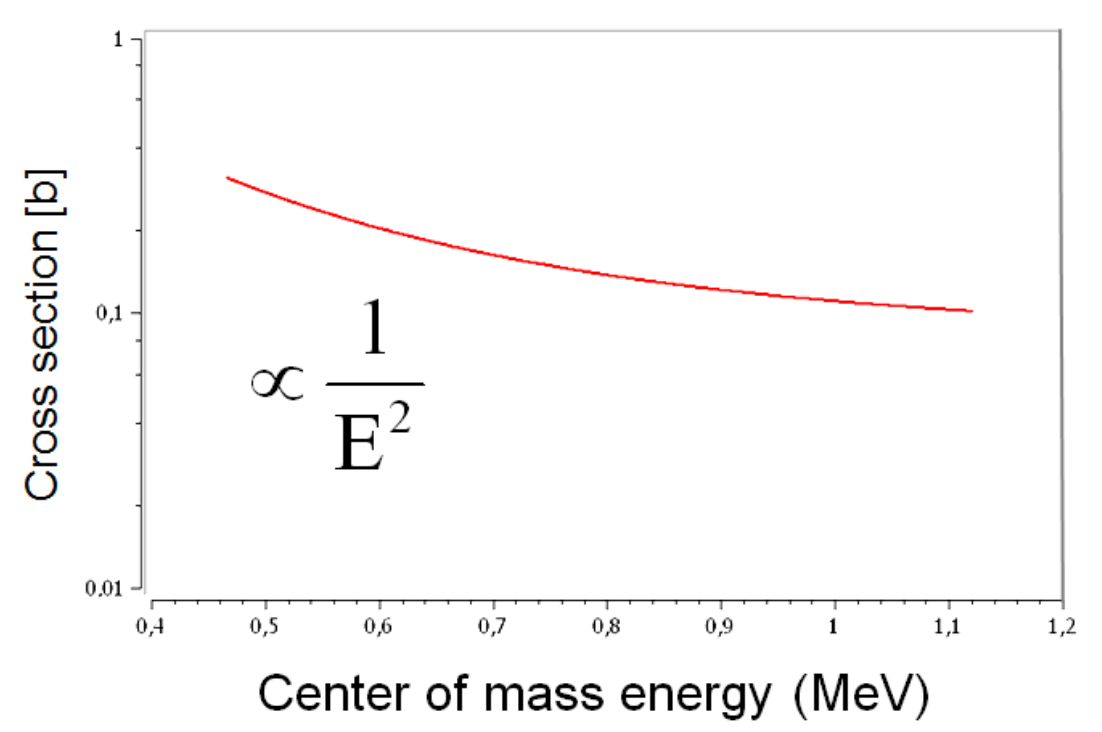
\includegraphics[width=0.65\linewidth]{captures/Capture.png}
		\caption{سطح مقطع دیفرانسیلی بر حسب انرژی در پراکندگی رادرفورد توسط نیروی دافعه‌ی کلمبی}
		\label{fig:diffcross}
	\end{figure}
	زمانی که این آزمایش توسط رادرفورد (1919) و چادویک (1921) برای ورقه‌های مختلف انجام شد، در بعضی نقاط نمودار، رزونانسی مشاهده کردند که با تئوری رادرفورد در تناقض بود.
	\begin{figure}[h]
		\centering
		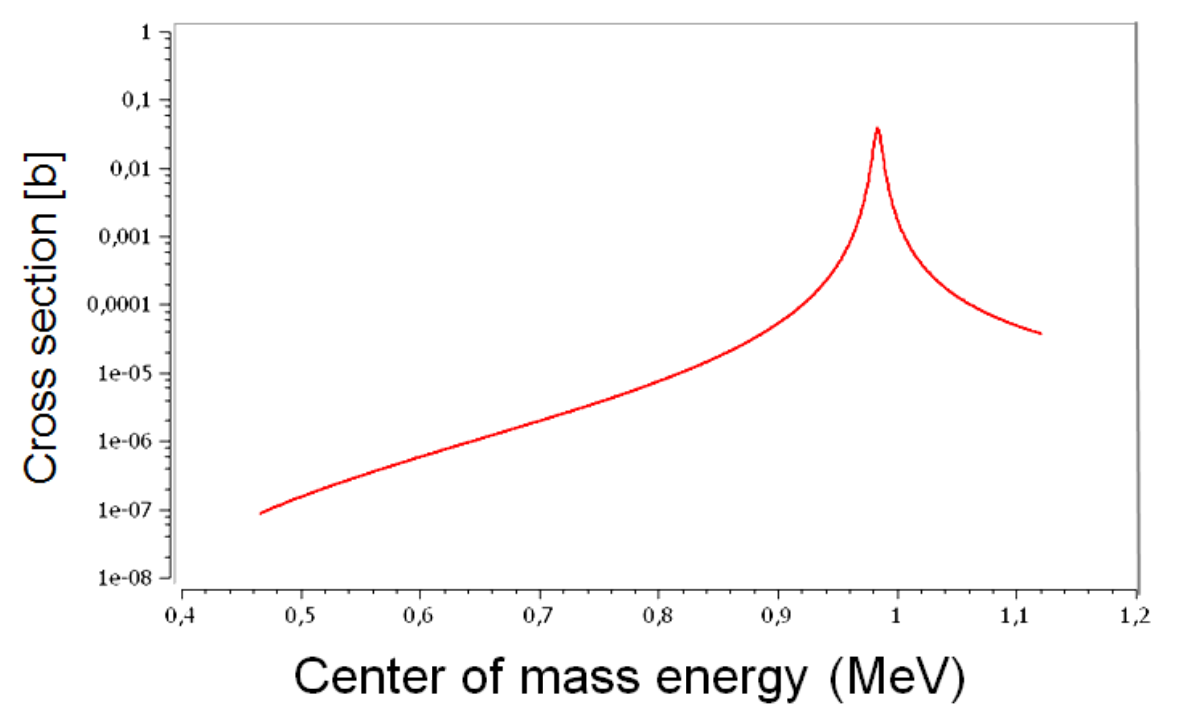
\includegraphics[width=0.65\linewidth]{captures/Capture1.png}
		\caption{رزونانس در نمودار سطح مقطع دیفرانسیلی بر حسب انرژی در پراکندگی الاستیک}
		\label{fig:reso}
	\end{figure}
	
	دلیل این رزونانس‌ها، وجود ذراتی در این آزمایش بودند که انرژی آن برای هر ذره مشخص است و هرچقدر این انرژی بیشتر باشد، تفاوت آزمایش و تئوری بیشتر می شود.
	\begin{figure}[h]
		\centering
		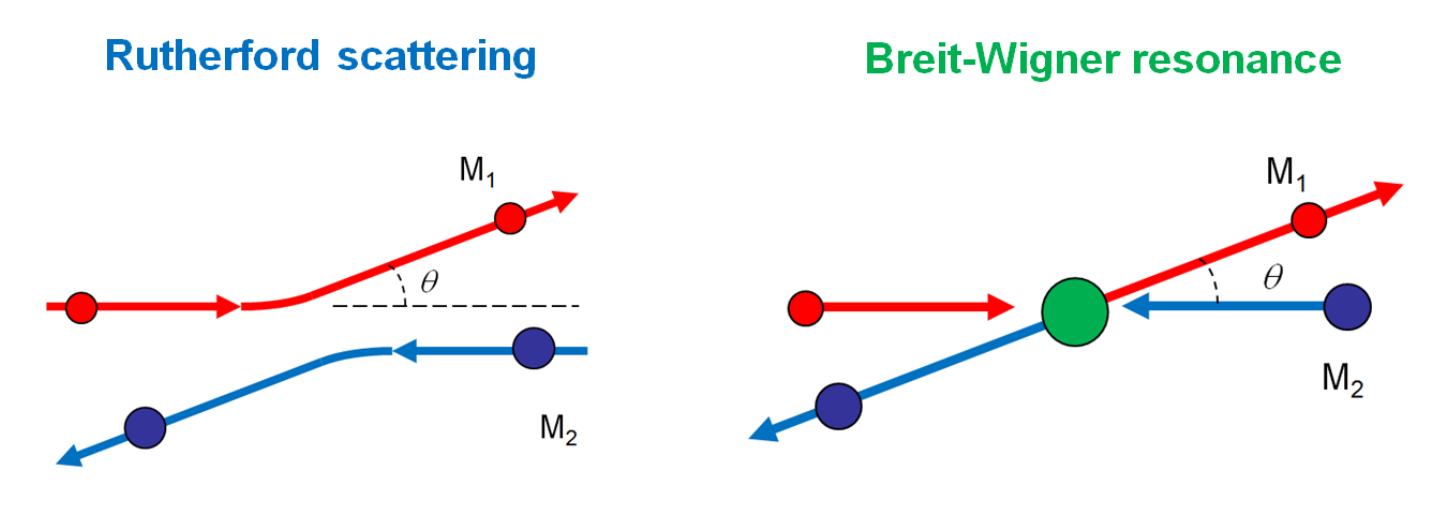
\includegraphics[width=\linewidth]{captures/Capture2.png}
		\caption{وجود ذره در پراکندگی الاستیک}
	\end{figure}
	
	اگر در محدوده‌ی بزرگتری از انرژی به سطح مقطع دیفرانسیلی نگاه کنیم، مشاهده می‌کنیم که در بازه‌ای از انرژی، سطح مقطع دیفرانسیلی با عکس مجذور انرژی رابطه
	دارد و با تئوری رادرفورد مطابقت دارد و با نزدیک شدن به محدوده‌ای از انرژی، رزونانس مشاهده می‌شود. در واقع تصویر 
	\ref{fig:reso}
	بخشی از نمودار اصلی است.
	\begin{figure}[h]
		\centering
		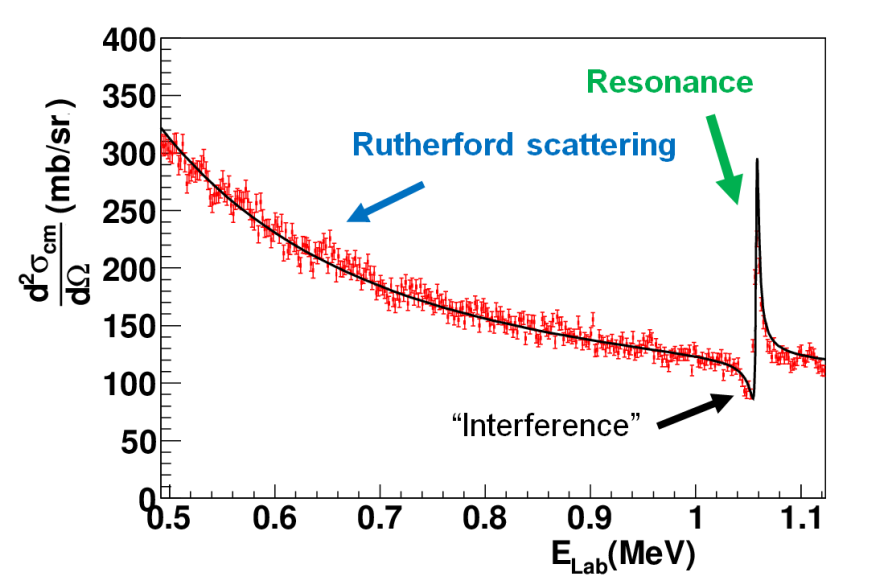
\includegraphics[width=\linewidth]{captures/Capture3.png}
		\caption{سطح مقطع دیفرانسیلی بر حسب انرژی ذرات آلفا در وجود 
			${}^{15}O$
		}
	\end{figure}
	
	دلیل رزونانس این است که ذره فرستاده‌شده و ذره موجود با هم ادغام می‌شوند  و هسته‌ی جدیدی می سازند که به شدت ناپایدار است و به صورت پراکندگی الاستیک واپاشی
	می‌کنند. این آزمایش در ابتدا با اتم های سنگین بررسی شد ولی بعدا در فیزیک ذرات بنیادی برای محاسبه‌ی جرم و طول عمر ذرات که مقادیر بسیار کوچکی هستند نیز
	استفاده شد.
	
	اگر به جای اکسیژن ذره ای بنیادی داشته باشیم، با مشاهده ی انرژی ای که رزونانس در آن رخ می‌دهد، می‌توان جرم ذره را محاسبه کرد. یکی از روش‌های محاسبه‌ی
	طول عمر ذرات به این صورت است که  با انجام آزمایش، هیستوگرامی از جرم های بدست آمده از رزونانس ها رسم کرده و با استفاده از آن، طول عمر ذره را بدست آورد.
	
	یکی از روش های دیگر، بررسی احتمال رخ دادن رزونانس در انرژی $E$ است که به تابع توزیع چگالی احتمال نسبیتی بریت-ویگنر معروف است و
	با رابطه زیر داده می‌شود\cite{breit_wigner_1936}:
	
	\begin{equation}
		f(E) = \frac{k}{\left(E^2-M^2\right)^2+M^2\Gamma^2}
	\end{equation}
	که $E$ در آن انرژی مرکز جرم، $M$ جرم ذره‌ی عامل رزونانس، $\Gamma$ عرض بازه‌ای که رزونانس دیده می‌شود و همین‌طور
	$k$ در آن به صورت زیر تعریف می شود:
	\begin{equation}
		k = \frac{2 \sqrt{2} M \Gamma  \gamma }{\pi \sqrt{M^2+\gamma}}   \quad  , \quad     \gamma=\sqrt{M^2\left(M^2+\Gamma^2\right)}
	\end{equation}
	
	با استفاده از عرض رزونانس، رابطه‌ی طول‌عمر ذره در دستگاه SI به صورت زیر خواهد شد:
	\begin{equation}
		\tau=\frac{\hbar}{\Gamma}
	\end{equation}

	\section{بقای انرژی و ذرات تولید شده در واپاشی}
	با توجه به بقای تکانه و بقای انرژی، اگر $E_i$ و $\vb{p}_i$ به ترتیب انرژی و تکانه ذره $i$م تولید شده در واپاشی باشد، انرژی و تکانه ذره واپاشی شده از
	روابط زیر بدست می‌آید:
	\begin{align}
		E &= \sum_i E_i \\
		\vb{p} &= \sum_i \vb{p}_i
	\end{align}
	همچنین طبق رابطه جرم-انرژی اینشتین
	\begin{equation}
		E^2 = m^2c^4 + p^2c^2
	\end{equation}
	پس جرم سکون ذره برابر است با
	\begin{equation}
		m = \sqrt{\qty(\sum_i E_i)^2 - \qty(\sum_i p_i)^2c^2}.
	\end{equation}

	در یک آزمایش واپاشی، با بدست آوردن $m$ از رابطه بالا، توزیع جرم سکون مشابه شکل \ref{fig:jpsi_hist_full} و \ref{fig:z0_hist_full} بدست می‌آوریم. در این
	نمودارها به نظر می‌رسد پیک نزدیک $\SI{3}{\giga\electronvolt}$ در نمودار اول و پیک نزدیک $\SI{90}{\giga\electronvolt}$ در نمودار دوم نشان دهنده ذره هستند.
	به طور خاص، در اینجا به ترتیب واپاشی ذرات $J/\psi$ و $Z^0$ به دو میون ($\mu$) را داریم. با جدا کردن پیک و محاسبه انحراف معیار جرم‌ها در نزدیکی آن،
	می‌توانیم $\Delta{m}$ مورد نیاز برای محاسبه طول‌عمر از اصل عدم قطعیت را بدست آوریم. با این روش، طول عمرهای بدست آمده برابرند با
	\begin{align}
		\tau(J/\psi) &\approx \num{9e-24}  \\
		\tau(Z^0) &\approx \num{1.4e-25}
	\end{align}
	از طرفی، طول‌عمرهای میانگین گزارش شده برای این ذرات برابرند با
	\begin{align}
		\tau(J/\psi) &\approx \num{7.2e-21}  \\
		\tau(Z^0) &\approx \num{3e-25}
	\end{align}
	برای بوزون $Z^0 $ مرتبه بزرگی طول‌عمر را به درستی بدست آوردیم، اما طول‌عمر محاسبه شده برای مزون $J/\psi$ اختلاف زیادی با عدد واقعی دارد. دلیل اختلاف
	اعداد ما با اعداد گزارش شده این است که ما برای این ذرات فقط یک حالت واپاشی را بررسی کردیم (واپاشی به دو میون):
	\begin{align}
		J/\psi &\longrightarrow \mu^{+} + \mu^{-} \\
		Z^0 &\longrightarrow \mu^{+} + \mu^{-}
	\end{align}
	برای $Z^0 $، با اینکه این مکانیزم فقط مربوط به سه درصد واپاشی‌هاست، زمان بقیه واپاشی‌ها مشابه همین است و به همین دلیل با دقت بهتری طول‌عمر را بدست آوردیم.
	اما برای $J/\psi$ واپاشی‌های بسیار کُندتری نیز وجود دارد که به این واپاشی غلبه می‌کنند (این مکانیزم فقط مربوط به شش درصد واپاشی‌هاست).
	
	برای مطالعه بیشتر، می‌توانید به آموزش‌های سایت \url{opendata.cern.ch} مراجعه کنید.

	\begin{figure}[h]
		\centering
		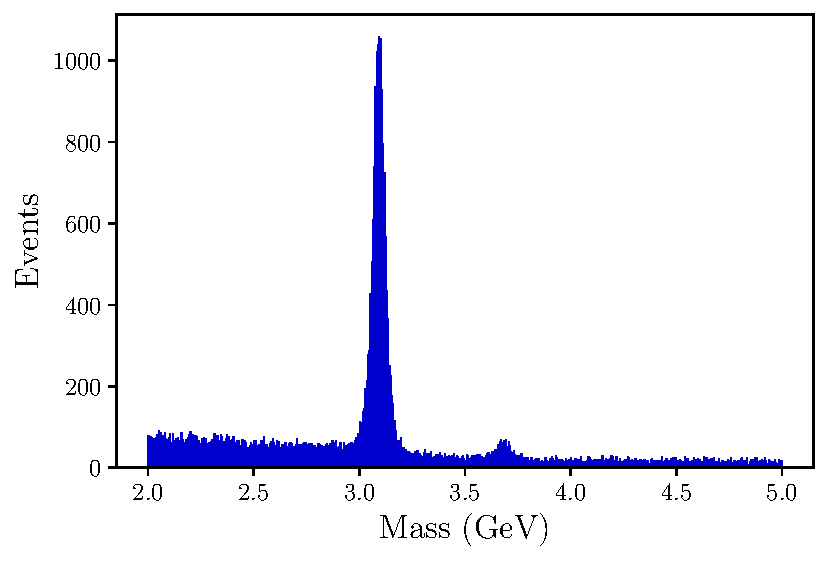
\includegraphics[width=0.85\linewidth]{calculations/jpsi_full_mass_hist.pdf}
		\caption{هیستوگرام جرم سکون در واپاشی $J/\psi$ به دو میون. استخراج شده از داده‌های سِرن در \url{opendata.cern.ch}}
		\label{fig:jpsi_hist_full}
	\end{figure}
	\begin{figure}[h]
		\centering
		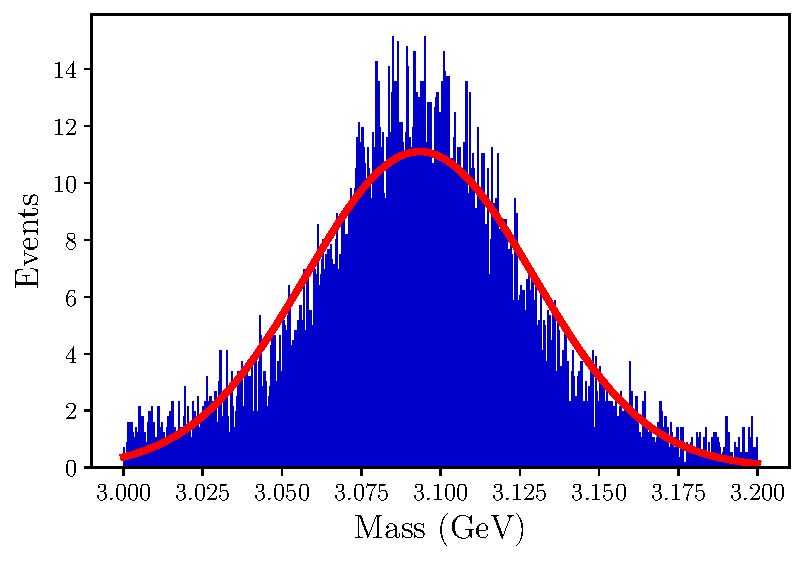
\includegraphics[width=0.85\linewidth]{calculations/jpsi_peak_mass_hist.pdf}
		\caption{پیک جرم سکون در واپاشی $J/\psi$ به دو میون}
	\end{figure}
	\begin{figure}[h]
		\centering
		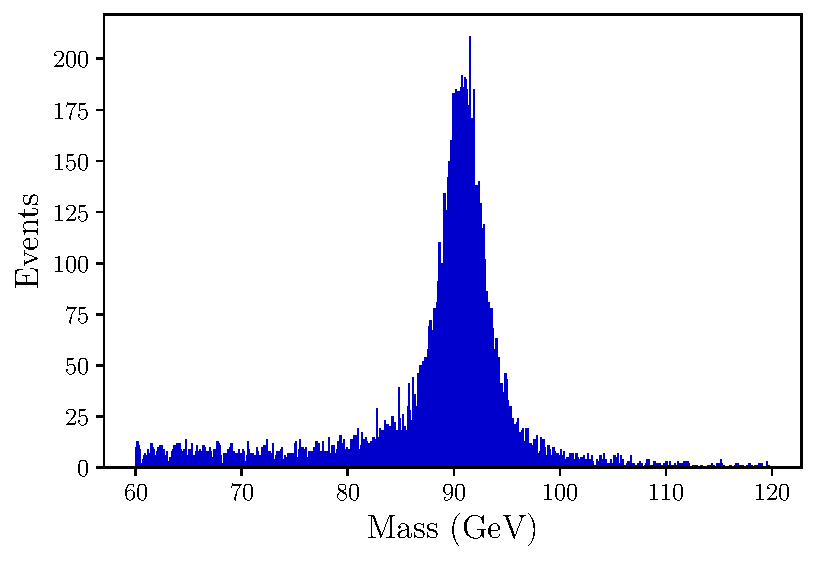
\includegraphics[width=0.9\linewidth]{calculations/z0_full_mass_hist.pdf}
		\caption{هیستوگرام جرم سکون در واپاشی $Z^0$ به دو میون. استخراج شده از داده‌های سِرن در \url{opendata.cern.ch}}
		\label{fig:z0_hist_full}
	\end{figure}
	\begin{figure}[h]
		\centering
		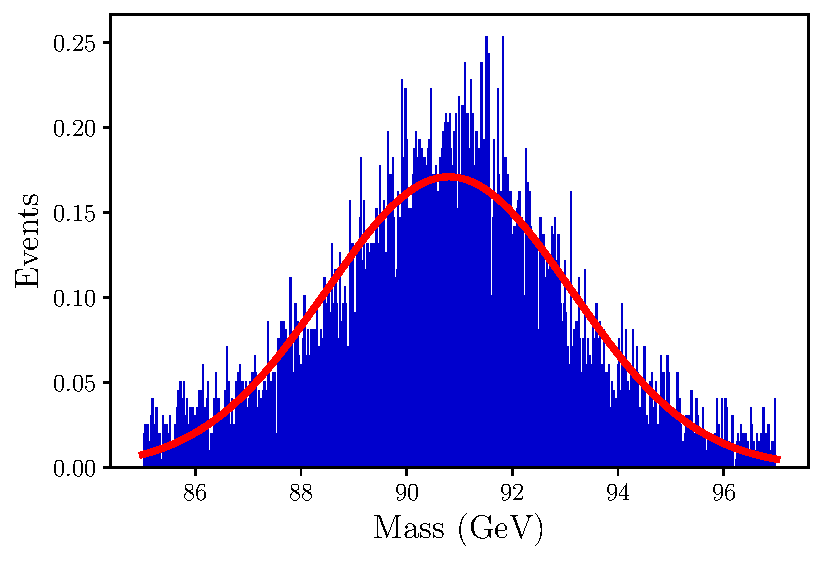
\includegraphics[width=0.9\linewidth]{calculations/z0_peak_mass_hist.pdf}
		\caption{پیک جرم سکون در واپاشی $Z^0$ به دو میون}
	\end{figure}

	\section{اعتبار روش‌ها}
	از آنجا که این روش‌ها غیرمستقیم هستند و به طور دقیق با مفهوم اندازه‌گیری زمان منطبق نیستند، شاید برای شما قانع‌کننده نباشند. اندازه‌گیری زمان در تعریف
	کلاسیکی، توسط مقایسه با یک پدیده متناوب انجام می‌شود؛ به عنوان مثال، بنا به تعریف ۲۴ ساعت طول می‌کشد تا خورشید به مکان قبلی خود در آسمان برگردد و با
	مقایسه زمان در روز با این پدیده تکرارشونده، ساعت را تعریف می‌کنیم و اندازه‌گیری می‌کنیم یک پدیده چند «ساعت»، یا چه نسبتی از این پدیده تکرارشونده
	طول می‌کشد. در تعریف جدیدِ زمان نیز تعداد نوسانات اتم سزیم اندازه‌گیری می‌شود، اینکه چه تعداد از این «تناوب‌ها» در طول یک پدیده اتفاق می‌افتد.
	
	روش‌های ذکرشده در این مقاله، از این جنس اندازه‌گیری‌ها نیستند، اما می‌دانیم در بازه‌های زمانی دیگر منطبق بر تعریف کلاسیکی هستند. دلیلی وجود ندارد
	که فکر کنیم در بازه‌های زمانی	دیگر، این روش بر تعریف موردنظر ما از زمان منطبق نباشد. اما در همینجا به این مشکل می‌خوریم که اصلاً تعریف کلاسیکی
	ما از زمان در توصیف طول‌عمر ذرات سودمند است یا نه. از ابتدا مفهوم مورد نظر ما کوانتومی است، پس نیاز به تعریف کوانتومی از طول‌عمر داریم.
	در واقع تعریفی از زمان که در اندازه‌گیری طول‌عمر ذرات انرژی بالا استفاده می‌کنیم، تعمیم تعریف کلاسیکی آن برای پدیده‌های کوانتومی است.
	طول‌‌عمر ذرات معیاری از پایداری آن‌ها است، و زمان مورد نیاز برای تغییر حالت کوانتومی آن، دقیقاً همین را به ما نشان می‌دهد.
	\setLTRbibitems
	\bibliographystyle{plain}
	\bibliography{ref}
\end{document}
